\documentclass[12pt,a4paper,draft]{article}
\usepackage{cmap}
\usepackage[utf8]{inputenc}
\usepackage[T2A]{fontenc}
\usepackage[english,german,russian]{babel}
\usepackage{amsmath}
\usepackage{amsfonts}
\usepackage{amssymb}
\usepackage[final]{graphicx}
\DeclareGraphicsExtensions{.jpg,.png}
\graphicspath{{pictures/}} % путь к графическим файлам. Пусть они помещаются в подкаталог pictures текущего каталога
\usepackage[figurename=Рисунок,labelsep=period]{caption}
\usepackage{float}
\usepackage{indentfirst}
\usepackage[pdftex,left=2.5cm,right=2.5cm,top=3cm,bottom=3cm]{geometry}
\usepackage[obeyDraft]{todonotes}
\usepackage[hidelinks,draft=false]{hyperref}
\frenchspacing
\pdfcompresslevel=9

\begin{document}

\def\contentaname{Содержание}
\tableofcontents %Вывод содержания
\clearpage

\section{Введение}
    Компьютерная графика - использование вычислительной техники для создания графических изображений, их отображения различными средствами и манипулирования ими.

    Виды компьютерной графики:
    \begin{enumerate}
        \item
        \begin{itemize}
          \item{Растровая графика}
          \item{Векторная графика}
          \item{Фрактальная графика}
        \end{itemize}
        \item
        \begin{itemize}
          \item{Двухмерная графика}
          \item{Трёхмерна (3D) графика}
        \end{itemize}
    \end{enumerate}

\section{Аналитический раздел}
    Для постоения реальстичной модели необходимо учитывать следующие физические аспекты:
    \begin{itemize}
      \item приломление света объектами
      \item поглощение (абсорбация) света жидкостью
    \end{itemize}
    \subsection{Закон преломление света Волновая оптика}

    Преломление света — явление, при котором луч света, переходя из одной среды в другую, изменяет направление на границе этих сред.

    \begin{figure}[H]%Картинка для закона преломления света
        \noindent\centering{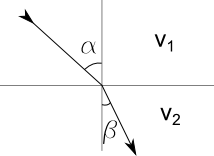
\includegraphics[scale = 1]{h55_1}}
        \caption{Закон приломления света}
        %\label{zakon_prilomleniya}
    \end{figure}

    Преломление света происходит по следующему закону:
    Падающий и преломленный лучи и перпендикуляр, проведенный к границе раздела двух сред в точке падения луча, лежат в одной плоскости. Отношение синуса угла падения к синусу угла преломления есть величина постоянная для двух сред:

    \begin{equation}%формула закона преломления света
        %\label{koef_prilom}
        n = \frac{\sin(\alpha)}{\sin(\beta)} = \frac{v_1}{v_2}
    \end{equation}

    где $\alpha$  угол падения,$\beta$  угол преломления,n  постоянная величина, не зависящая от угла падения.

    При изменении угла падения изменяется и угол преломления. Чем больше угол падения, тем больше угол преломления.

    Если свет идет из среды оптически менее плотной в более плотную среду, то угол преломления всегда меньше угла падения: $\beta < \alpha$.

    Луч света, направленный перпендикулярно к границе раздела двух сред, проходит из одной среды в другую без преломления.

    \subsubsection{Показатель преломления}
        Физический смысл относительного показателя преломления (иначе показателя преломления второй среды относительно первой): он показывает во сколько раз скорость света в той среде, из которой луч выходит, больше скорости света в той среде, в которую он входит.

        \begin{equation}
            %\label{koef_prilom1}
            n = \frac{\sin(\alpha)}{\sin(\beta)} = \frac{v_1}{v_2} = \frac{n_2}{n_1}
        \end{equation}

        Кроме того, каждая среда, через которую проходит луч света, характеризуется абсолютным показателем преломления:

        \begin{equation}
            %\label{koef_prilom1}
            n = \frac{c}{v_1}
        \end{equation}

        Абсолютный показатель преломления - это показатель преломления среды относительно вакуума. Он равен отношению скорости света в вакууме к скорости света в данной среде.
        Среда с меньшим абсолютным показателем преломления называется оптически менее плотной средой.

    \subsubsection{Преломление в плоскопараллельной пластине.}
        Проследим ход луча через прозрачную пластину с параллельными гранями.

        \begin{figure}[H]%Картинка для закона преломления света
            \noindent\centering{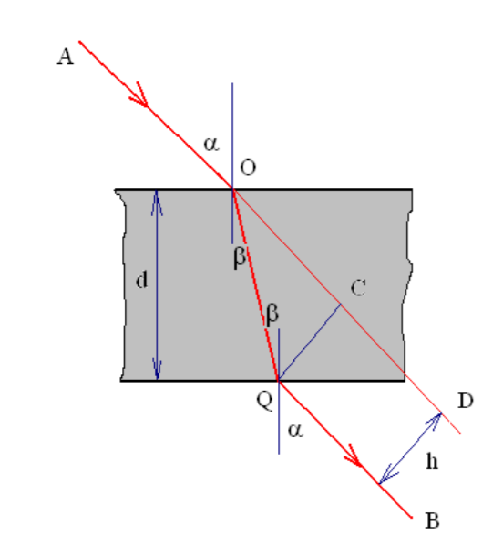
\includegraphics[scale = 1]{plastina}}
            \caption{Преломление в плоскопараллельной пластине}
            %\label{zakon_prilomleniya}
        \end{figure}

        Падающий на пластину луч, после двукратного преломления в точках О и Q, выйдет из пластины (вследствие обратимости световых лучей) параллельно падающему лучу АО, смещенный на расстояние h. Найдем величину смещения, если d - толщина пластины.

        \begin{equation}
            \label{rasst}
            h = QC = OC\sin(\alpha-\beta) = \frac{d\sin(\alpha-\beta)}{\cos\beta}
        \end{equation}



    \subsection{Поглощение (абсорбция) света}
    Поглощением (абсорбцией) света называется явление потери энергии световой волной, проходящей через вещество.

    Свет поглощается в тех случаях, когда проходящая волна затрачивает энергию на различные процессы. Среди них:
    \begin{itemize}
        \item преобразование энергии волны во внутреннюю энергию – при нагревании вещества;
        \item затраты энергии на вторичное излучение в другом диапазоне частот (фотолюминесценция);
        \item затраты энергии на ионизацию – при фотохимических реакциях;
        \item т.п.
    \end{itemize}

    Интенсивность волны будет изменяться по закону Бугера (П. Бугер (1698 – 1758) – французский ученый):

    %\begin{equation}
      %J(x) = J_0e^{\alpha x}
    %\end{equation}

    %где $x$ - толщина поглощающего слоя, $J_0$ – интенсивность волны на входе в среду, $\alpha$ - коэффициент поглощения, зависящий от длины волны света, химической природы и состояния вещества и не зависящий от интенсивности света при слабых световых потоках.

    %На рисунке представлена типичная зависимость коэффициента поглощения от длины волны света. Зависимостью коэффициента поглощения от \lambda объясняется окрашенность поглощающих тел. Например, стекло, слабо поглощающее красные и оранжевые лучи и сильно поглощающее зеленые и синие, при освещении белым светом будет казаться красным. Если на такое стекло направить зеленый и синий свет, то из-за сильного поглощения света этих длин волн стекло будет казаться черным. Зависимость коэффициента поглощения от длины волны света используется для изготовления светофильтров, которые в соответствии с химическим составом пропускают свет только определенных длин волн, поглощая остальные. 

    \begin{figure}[H]%Картинка для закона преломления света
            \noindent\centering{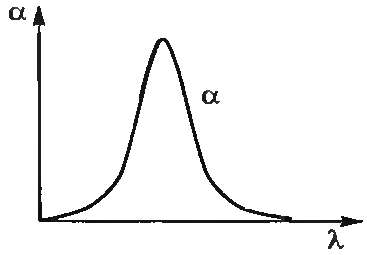
\includegraphics[scale = 1]{absorb}}
            \caption{Преломление в плоскопараллельной пластине}
            %\label{zakon_prilomleniya}
        \end{figure}

\end{document} 